\documentclass[11pt,onecolumn,letterpaper]{article}
\usepackage{amsmath,amssymb,graphicx,algorithmic,xspace,url,latexsym}

\usepackage[parfill]{parskip}
\usepackage{paralist}
\usepackage{times}
\usepackage{textcomp}
\usepackage{hyperref}
\usepackage{listings}
\usepackage{color}

\usepackage{makeidx}
\makeindex

\setlength{\evensidemargin}{-0.1in} \setlength{\oddsidemargin}{-0.1in}
\setlength{\textwidth}{6.5in} \setlength{\textheight}{9.0in}
\setlength{\topmargin}{-0.5in}
%\setlength{\headheight}{0in}

\newcounter{qNum}
\setcounter{qNum}{1}
\newcommand{\q}[1]{\vspace*{0.15in} \noindent
\arabic{qNum}.(#1 points)~\stepcounter{qNum}}

\newcommand{\main}{\(Main\)}
\newcommand{\lib}{\(Lib\)}
\newcommand{\set}[1]{\{#1\}}

\newcommand{\js}{JavaScript}
\newcommand{\dl}{\texttt{DOLOTO}}

\newtheorem{theorem}{Theorem}

\newcommand{\EmbedCode}[3]{
	\lstset{language=#1, frame=none, backgroundcolor=\color{white},
			rulecolor=, xleftmargin=5.0ex}
	%\lstset{linewidth=\columnwidth}
	\lstset{commentstyle=\textit, stringstyle=\upshape,showspaces=false}
	\lstset{frame=none, showstringspaces=false, numbers=#3,
			numberblanklines=false}
	\lstinputlisting[]{#2} 
}

\sloppypar
\begin{document}
\pagestyle{empty}

\author{Xavier NOUMBISSI}

\begin{center}
\begin{large}
XAVIER NOUMBISSI\\
xnoumbis@uwaterloo.ca\\
\vspace{0.5cm}
ECE 750: Static Analysis for Software Engineering\\
\vspace{0.5cm}
Final Exam
\end{large}

\end{center}
\section*{Question 1}

\begin{enumerate}[(a)]
\item Symbolic Heap for function \texttt{f} in Example 6

\begin{figure}[!ht]
\centering
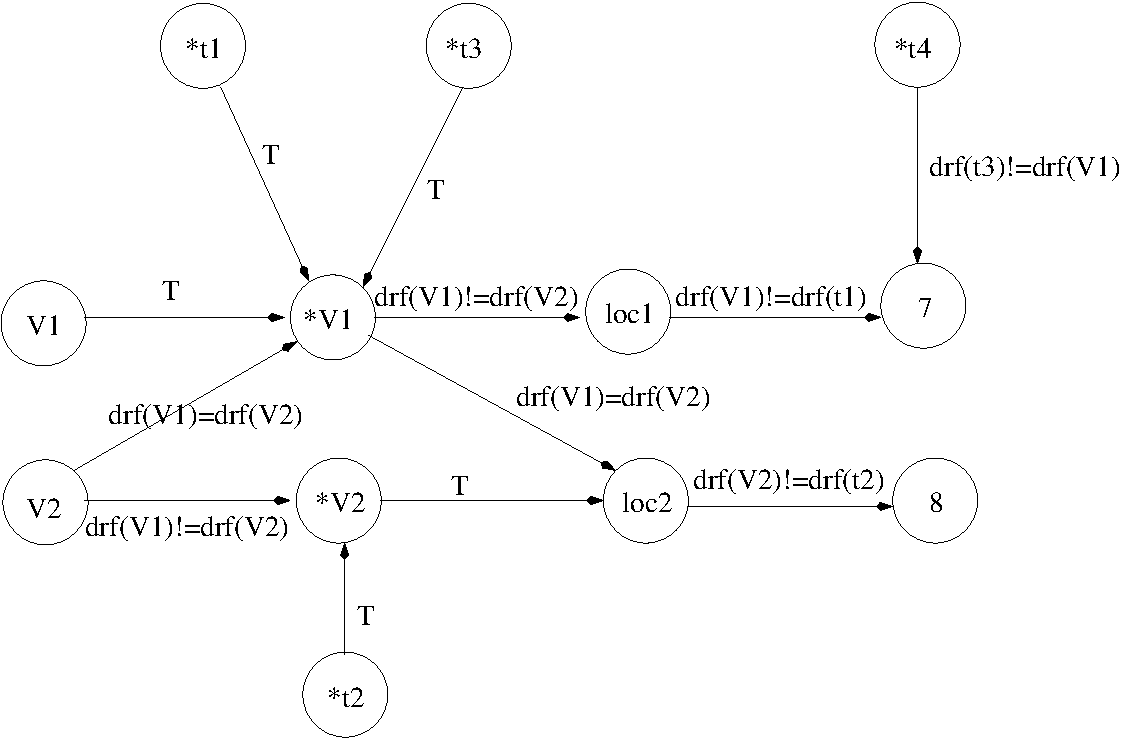
\includegraphics[scale=0.8]{q1-heap.pdf}
\label{fig:symheap}
\end{figure}

\item Precondition for function \texttt{g}: $\mathit{drf}(v1) \neq \mathit{drf}(v2) $

The precondition stipulates that formal parameters $a1$ and
$a2$ of \texttt{d} must not alias before entering \texttt{g}.

\item Summary for function \texttt{g}

\begin{figure}[!ht]
\centering
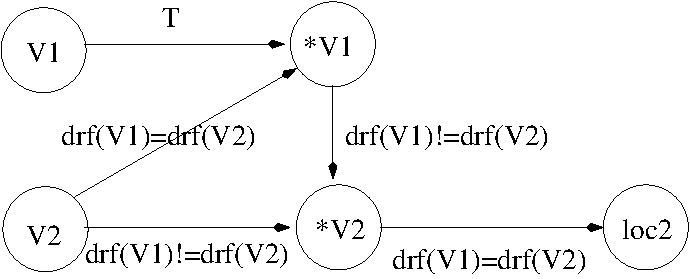
\includegraphics[scale=0.8]{q1-sum.pdf}
\label{fig:symheap}
\end{figure}

\end{enumerate}
\newpage

\section*{Question 2: Application of Techniques from \cite{Pradel:2013:ATS}}

\newcommand{\myA}{\texttt{A}}
\newcommand{\myB}{\texttt{B}}

Given class \myA{} and its subclass \myB{} from the exam
sheet, we are going to show that class \myB{} is a
\textit{crashing substitute} of its super class \myA{}.

\paragraph*{Constructor Mapping}
Given the fact that the subclass (\myB{}) and the super
class (\myA{}) do not have the exact same types of arguments,
we define the following constructor mapping that show the
equivalence between constructor calls of \myB{} and \myB{}.

$\mathit{B}(int) \rightarrow \mathit{A}()$

\paragraph*{Test Generation}
According to 
\newpage

\section*{Question 3: Paper Summary of "Automatic Testing of Sequential and Concurrent Substitutability"}

\newcommand{\mysub}{substitutability}
\newcommand{\mySub}{Substitutability}

\paragraph{Key Ideas.}
The paper addresses the problem of \textit{\mysub} in 
object-oriented programming languages. \textit{\mySub} is relevant
for languages featuring \textit{polymorphism} and \textit{inheritance}.
The \mysub{} principle stipulates that a subclass of an upper
class shall be safely used whenever it is accessed from a
pointer that has the type of the upper class. That is, it is
semantically safe to use a subclass instance everywhere an
upper class instance could be used.

The authors present a testing technique that helps checking
that code preserves the \mysub{} principle. Their technique
can be used for both sequential and concurrent programs.
Given a class \textit{Super} and its subclass \textit{Sub}, the
presented analysis generates test cases that can test both
\textit{Super} and \textit{Sub} instances. Then, the analysis
uses \textit{Super}'s behavior as an oracle for \textit{Sub}.
The analysis reports a warning whenever \textit{Sub} behaves
differently from \textit{Super}. The analysis comes in two
flavors: it can report any observed divergence between \textit{Super}
and \textit{Sub} or can report only cases when the divergence 
leads to a crash of the application.

The generated tests consist in a sequence of method calls,
specified by their name, their input parameter, and their
output variable if any. The tests are randomly created by
a test generator that can produce both sequential and
concurrent tests. The authors use the Java Pathfinder
model checker to explore all interleavings when running
tests to find unsafe \mysub{} in concurrent programs.

\paragraph{Justifications.}


\paragraph{Our opinion.}
The respect of \mysub{} is important for building correct
object-oriented systems. The tool presented by the paper
is therefore very useful to check semantic consistency of
object-oriented software.

The handling of concurrency by the authors is very relevant and
of great importance given the current ubiquitousness of
multi-core architectures.

\paragraph{Discussion Topics.}
\begin{itemize}
\item Since \dl{} adds more code (e.g., stubs) to an existing application, users
may eventually end downloading more data, thus increasing network usage and
costs. For what type of applications would \dl{} still be profitable to 
users ?

\end{itemize}

\newpage

\section*{Question 4: Invariant Generation as in \cite{Nguyen:2012:UDA}}


\newpage

\section*{Question 5}

\subsection*{Introduction}
This paper presents an intraprocedural analysis that detects
array accesses for which index variable checking was not done
on some paths leading to the access.

Statically verifying that programs check array index variables
before array accesses is useful at it may help developers detect
incorrect array accesses that may lead to program termination
at runtime.

EXAMPLE

Our analysis is implemented in the
Clang framework\footnote{http://clang-analyzer.llvm.org/},
which is a static source code analysis tool to find bugs in
C, C++, and objective C.

\subsection*{Intraprocedural Analysis}
%\bibliographystyle{plain}
%\bibliography{ctaint-proposal}

The Clang analyzer performs a symbolic execution on the CFG
of the program under analysis. The analysis is path- and
context-sensitive. To comply to the clang framework, we need
to implement our analysis as a \textit{checker}. 









\newpage

%%%%%%%%%%%%%%%%%%%%%%%%%%%%%%%%%%%%%%%%%%%%%%%%%%%%%%%%%%%%%%%%%%%%%%%%%%%%%%%%%%

\bibliographystyle{plain}
\bibliography{finalexam}

\end{document}
